
\documentclass[xcolor=pdftex,dvipsnames,table,mathserif,aspectratio=169]{beamer}
\usetheme{default}
\usetheme{metropolis}
\usepackage{ulem}
\usepackage{minted}
\usepackage{mathtools}
\setbeamersize{text margin left=.3in,text margin right=.3in} 

\DeclarePairedDelimiter\abs{\lvert}{\rvert}%
\DeclarePairedDelimiter\norm{\lVert}{\rVert}%


%\usetheme{Darmstadt}
%\usepackage{times}
%\usefonttheme{structurebold}

\usepackage[english]{babel}
%\usepackage[table]{xcolor}
\usepackage{pgf,pgfarrows,pgfnodes,pgfautomata,pgfheaps}
\usepackage{amsmath,amssymb,setspace,centernot}
\usepackage[latin1]{inputenc}
\usepackage[T1]{fontenc}
\usepackage{relsize}
\usepackage{pdfpages}
\usepackage[absolute,overlay]{textpos} 


\newenvironment{reference}[2]{% 
  \begin{textblock*}{\textwidth}(#1,#2) 
      \footnotesize\it\bgroup\color{red!50!black}}{\egroup\end{textblock*}} 

\DeclareMathSizes{10}{10}{6}{6} 

\begin{document}
\title{Part 8: Program Evaluation (c)\\
Local Average Treatment Effects}
\author{Chris Conlon}
\institute{Applied Econometrics}
\date{\today}

\frame{\titlepage}



\begin{frame}{What about IV?}
Recall the simple IV estimator with $\beta_i = \beta$:
\begin{align*}
Y_i(0) &= \beta_0 + u_i(0)\\
Y_i(1) &= \beta_0 + \beta1 T_i +  u_i(1)\\
Y_i &= Y_{i0} + \beta_1 T_i  + \underbrace{[u_i(1) - u_i(0)]}_{\eta_i}
\end{align*}
We are interested in the \alert{treatment effect} $\beta_1 = Y_i(1) - Y_i(0)$
\begin{itemize}
\item But $E[\eta_i |  T_i] \neq 0$ because of \alert{selection problem}
\item IV $Z_i$ gives us $\beta_1 = \frac{Cov(Y_i,Z_i)}{Cov(T_i,Z_i)}$ if $Z_i$ is ``excluded''...
\item But what does that mean?
\end{itemize}
\end{frame}

\begin{frame}
\frametitle{What about IV?}
\begin{itemize}
\item Note the absence of direct path between $z \rightarrow y$. This is the \alert{exclusion restriction}.
\item The fact hat $z \rightarrow x$ is the \alert{relevance} condition.
\end{itemize}
\begin{center}
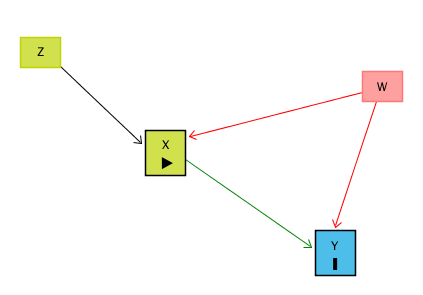
\includegraphics[width=3in]{./resources/dag-iv.png}
\end{center}

\end{frame}


\begin{frame}
\frametitle{So what does IV do?}
Now let's think about \alert{heterogeneous treatment effects} $\beta_i = Y_i(1) - Y_i(0)$
\begin{itemize}
\item Let's assume a binary instrument $Z_i=1$
\item $Y_i(1),Y_i(0)$ depends on the value of $T_i$
\item But now we allow $T_i(1),T_i(0)$ wher ehte argument is the value of $Z_i$
\item We observe $\{Z_i, T_i = T_i(Z_i), Y_i = Y_i(T_i(Z_i))\}$.
\item ``Reduced form'' is regression of $y_i \sim z_i$ or $E[Y_i | Z_i =1] - E[Y_i | Z_i =0]$\\
(Nothing about $T_i$!)
\end{itemize}
\end{frame}

\begin{frame}{IV Assumptions}
\textbf{Independence}: $Z_i \perp Y_i(1), Y_i(0), T_i(1), T_i(0)$. Instrument is as if randomly assigned and does not directly affect $Y_i$
\begin{itemize}
\item $T_i = T_i(0) + (T_i(1) - T_i(0)) Z_i$
\item Change in treatment status $(T_i(1) - T_i(0))$ is the causal effect of $Z_i$ on $T_i$
\item Under independence, the \alert{first stage} is the average causal effect of $Z_i$ on $T_i$
\begin{align*}
E[T_i | Z_i = 1] - E[T_i | Z_i = 0] 
&= E[T_i(1) | Z_i = 1] - E[T_i(0) | Z_i = 0]\\
&= E[T_i(1)-T_i(0)]
\end{align*}
\item This is not implied by random assignment. In that case there would be four potential outcomes $Y_i(z,t)$.
\end{itemize}
\end{frame}

\begin{frame}
\frametitle{IV Assumptions}
\begin{description}
\item [Independence] $Z_i \perp Y_i(1), Y_i(0), T_i(1), T_i(0)$.\\
 Instrument is as if randomly assigned and does not directly affect $Y_i$
\item [Random Assignment] $Z_i \perp Y_i(0,0), Y_i(0,1), Y_i(1,0), Y_i(1,1), T_i(1), T_i(0)$. 
\item [Exclusion Restriction] $Y_i(z,t) = Y_i(z',t)$ for all $z,z',t$. 
\end{description}
We require \alert{both RA and ER} to guarantee \textbf{Independence}.\\
The second assumption is a substantive one.
%\item We only observe $(Z_i,T_i)$ not the pair $T_i(0),T_i(1)$ so we cannot determine compliance types directly! (See the picture)
\end{frame}


\begin{frame}
\frametitle{IV Assumptions}
\begin{itemize}
\item Consider four possible pairs of $(t_i,z_i)$
\item Let $T_i(z_i)$ denote how treatment status responds to the instrument:
\end{itemize}

\begin{center}
\begin{tabular}{ r |  c c } 
 & \multicolumn{2}{c} {$T_{i}(0)$} \\
$T_{i}(1)$  & 0 & 1 \\
\hline 
 0 & never-taker & defier \\
 1 & complier & always-taker
\end{tabular}
\end{center}
\end{frame}



%
%
%\begin{frame}
%\frametitle{What about IV}
%So what does IV do?
%\begin{itemize}
%\item Let's assume a binary instrument $Z_i = 1$
%\item $Y_i(1),Y_i(0)$ depends on the value of $T_i$
%\item But now we endogenize $T_i(1) ,T_i(0)$ where the argument is the value of $Z_i$.
%\item We observe $\{Z_i, T_i = T_i(Z_i), Y_i = Y_i(T_i(Z_i)) \}$.
%\end{itemize}
%\end{frame}



\begin{frame}
\frametitle{IV Assumptions}
We are stuck without further assumptions, so we assume:
\begin{description}
\item [Monotonicity/No Defiers] $T_i(1) \geq T_i(0)$
\end{description}
\begin{itemize}
\item Works in many applications (classical drug compliance).
\item Implied by many latent index models with constant coefficients
\item Works as long as sign of $\pi_{1,i}$ doesn't change
\begin{eqnarray*}
T_i(z)  = 1 [\pi_0 + \pi_1 z + \varepsilon_i > 0]
\end{eqnarray*}
\end{itemize}
\end{frame}

\begin{frame}
\frametitle{IV Assumptions}
\alert{Monotonicity} rules out defiers
\begin{center}
\begin{tabular}{ r |  c c } 
 & \multicolumn{2}{c} {$T_{i}(0)$} \\
$T_{i}(1)$  & 0 & 1 \\
\hline 
 0 & never-taker & \sout{defier} \\
 1 & \alert{complier} & always-taker
\end{tabular}
\end{center}
The \alert{compliers} are the only group we learn about with the IV estimator.
\end{frame}


\begin{frame}
\frametitle{IV Assumptions (Updated)}
Compliance Types by Treatment and Instrument  $(t_i,z_i)$\\
\alert{Monotonicity} rules out defiers
\begin{center}
\begin{tabular}{ r |  c c } 
 & \multicolumn{2}{c} {$Z_i$} \\
$T_{i}$  & 0 & 1 \\
\hline 
 0 & complier/never-taker & never-taker/\sout{defier} \\
 1 & always-taker/\sout{defier} & complier/always-taker
\end{tabular}
\end{center}
\begin{align*}
\{ \text{treated} \} = \{ \text{always-takers} \} + & \{ \text{compliers assigned } z_i=1 \}\\
\{ \text{control} \} = \{ \text{never-takers} \}  + & \{ \text{compliers assigned } z_i=0 \}
\end{align*}
\end{frame}



\begin{frame}
\frametitle{LATE Theorem}
\begin{itemize}
\item We can derive the expression for $\beta_{IV}$ as the \alert{Wald Estimator}:
\begin{eqnarray*}
\beta_{IV} = \frac{E[Y_i  | Z_i = 1] - E[Y_i | Z_i = 0] }{E[T_i | Z_i=1 ] - E[T_i | Z_i = 0]} = E[Y_i(1) - Y_i(0) | \text{complier}]
\end{eqnarray*}
\item We can derive the expression for $\pi_c$ (the fraction of compliers):
\begin{eqnarray*}
\pi_c = E[T_i | Z_i = 1] - E[T_i | Z_i =0] 
\end{eqnarray*}
\item Proof see Angrist and Imbens
\end{itemize}
\end{frame}

\begin{frame}{Is this what we wanted?}
\begin{itemize}
\item We learn about the average treatment effect for the group of \alert{compliers}
\item Different people comply with different instruments
\begin{itemize}
\item Imagine two ways ot increase college attendance: \alert{merit scholarships} and \alert{financial aid}
\item Different instruments trace out different groups of \alert{compliers}
\end{itemize}
\item Is this what we want? Probably not.
\item Maybe it isn't that far away...?
\end{itemize}

\end{frame}



\begin{frame}
\frametitle{How Close to ATE?}
Angrist and Imbens give some idea how close to the ATE the LATE is:
\begin{itemize}
\item $E[Y_i(0) | \text{never-taker}]$ and  $E[Y_i(1) | \text{always-taker}]$ can be estimated from the data
\item Compare these to their respective compliers $E[Y_i(0) | \text{complier}]$, $E[Y_i(1) | \text{complier}]$.
\item When these are close then possibly $ATE \approx LATE$.
\end{itemize}
\end{frame}

\begin{frame}
\frametitle{How Close to ATE?}
Angrist and Imbens give some idea how close to the ATE the LATE is:
\begin{eqnarray*}
\widehat{\beta}_1^{TSLS} \rightarrow^p \frac{E[\beta_{1i} \pi_{1i}]}{E[\pi_{i1}]} = LATE \\
LATE = ATE + \frac{Cov(\beta_{1i},\pi_{1i})}{E[\pi_{1i}]}
\end{eqnarray*}
\begin{itemize}
\item Weighted average for people with large $\pi_{1i}$.
\item Late is treatment effect for those whose probability of treatment is most influenced by $Z_i$.
\item If you always (never) get treated you don't show up in LATE.
\end{itemize}
\end{frame}

\begin{frame}
\frametitle{How Close to ATE?}
\begin{itemize}
\item With different instruments you get different $\pi_{1i}$ and TSLS estimators!
\item Even with two valid $Z_1, Z_2$
\begin{itemize}
\item Can be influential for different members of the population.
\item Using $Z_1$, TSLS will estimate the treatment effect for people whose probability of treatment $X$ is most influenced by $Z_1$
\item The LATE for $Z_1$ might differ from the LATE for $Z_2$
\item A J-statistic might reject even if both $Z_1$ and $Z_2$ are exogenous! (Why?).
\end{itemize}
\end{itemize}
\end{frame}


\begin{frame}
\frametitle{Example: Cardiac Catheterization}
\begin{itemize}
\item $Y_i=$ surival time (days) for AMI patients
\item $X_i=$ whether patient received cadiac catheterization (or not) (intensive treatment)
\item $Z_i=$ differential distance to CC hospital
\end{itemize}
\begin{eqnarray*}
SurvivalDays_i &=& \beta_0 + \beta_{1i} CardCath_i + u_i\\
CardCath_i &=& \pi_0 + \pi_{1i} Distance_i + v_i
\end{eqnarray*}
\begin{itemize}
\item For whom does distance have the great effect on probability of treatment?
\item For those patients what is their $\beta_{1i}$?
\end{itemize}
\end{frame}


\begin{frame}
\frametitle{Example: Cardiac Catheterization}
\begin{itemize}
\item IV estimates causal effect for patients whose value of $X_i$ is most heavily influenced by $Z_i$
\begin{itemize}
\item Patients with small positive benefit from CC in the expert judgement of EMT will receive CC if trip to CC hospital is short (\alert{compliers})
\item Patients that need CC to survive will always get it (\alert{always-takers})
\item Patients for which CC would be unnecessarily risky or harmful will not receive it (\alert{never-takers})
\item Patients for who would have gotten CC if they lived further from CC hospital (hopefully don't see) (\alert{defiers})
\end{itemize}
\item We mostly weight towards the people with small positive benefits.
\end{itemize}
\end{frame}


\begin{frame}{Local Average Treatment Effect}
So how is this useful? 
\begin{itemize}
\item It shows why IV can be meaningless when effects are heterogeneous.
\item It shows that if the monotonicity assumption can be justified, IV
estimates the effect for a particular subset of the population.
\item In general the estimates are specific to that instrument and are not
generalisable to other contexts.
\item As an example consider two alternative policies that can increase
participation in higher education.
\begin{itemize}
\item Free tuition is randomly allocated to young people to attend college ($Z_1 = 1$ means that the subsidy is available).
\item The possibility of a competitive scholarship is available for free tuition ($Z_1 = 1$ means that the individual is allowed to compete for the scholarship).
\end{itemize}
\end{itemize} 
\end{frame}


\begin{frame}{Local Average Treatment Effect}
\begin{itemize}
\item Suppose the aim is to use these two policies to estimate the returns to college education. In this case, the pair $\{Y^1, Y^0\}$ are log earnings, the treatment is going to college, and the instrument is one of the two randomly allocated programs.
\item First, we need to assume that no one who intended to go to college will be discouraged from doing so as a result of the policy (monotonicity).
\item This could fail as a result of a General Equilibrium response of the policy; for example, if it is perceived that the returns to college decline as a result of the increased supply, those with better outside opportunities may drop out.
\end{itemize}
\end{frame}

\begin{frame}{Local Average Treatment Effect}
\begin{itemize}
\item Now compare the two instruments.
\item The subsidy is likely to draw poorer liquidity constrained students into college but not necessarily those with the highest returns.
\item The scholarship is likely to draw in the best students, who may also have higher returns.
\item It is not a priori possible to believe that the two policies will identify the same parameter, or that one experiment will allow us to learn about the returns for a broader/different group of individuals.
\end{itemize}
\end{frame}

\begin{frame}{A Classic Example}
\begin{itemize}
\item What is the effect of prices on quantity demanded?
\item But a regression of $Q_t  = \beta_0 + \beta_1 P_T + u_t$ is going to be flawed.
\item For one thing, how do we know that relationship represents supply or demand?
\item Imagine an instrument $Z_t \in \{0,1\}$ that reduces supply but does not effect demand.
\item What about?
\begin{itemize}
\item Monotonicity?
\item Heterogeneity in treatemnt effects?
\item Exclusion Restriction?
\end{itemize}
\end{itemize}
\end{frame}


\begin{frame}
\frametitle{LATE at the Fulton Fish Market (Graddy 1995)}

\begin{center}
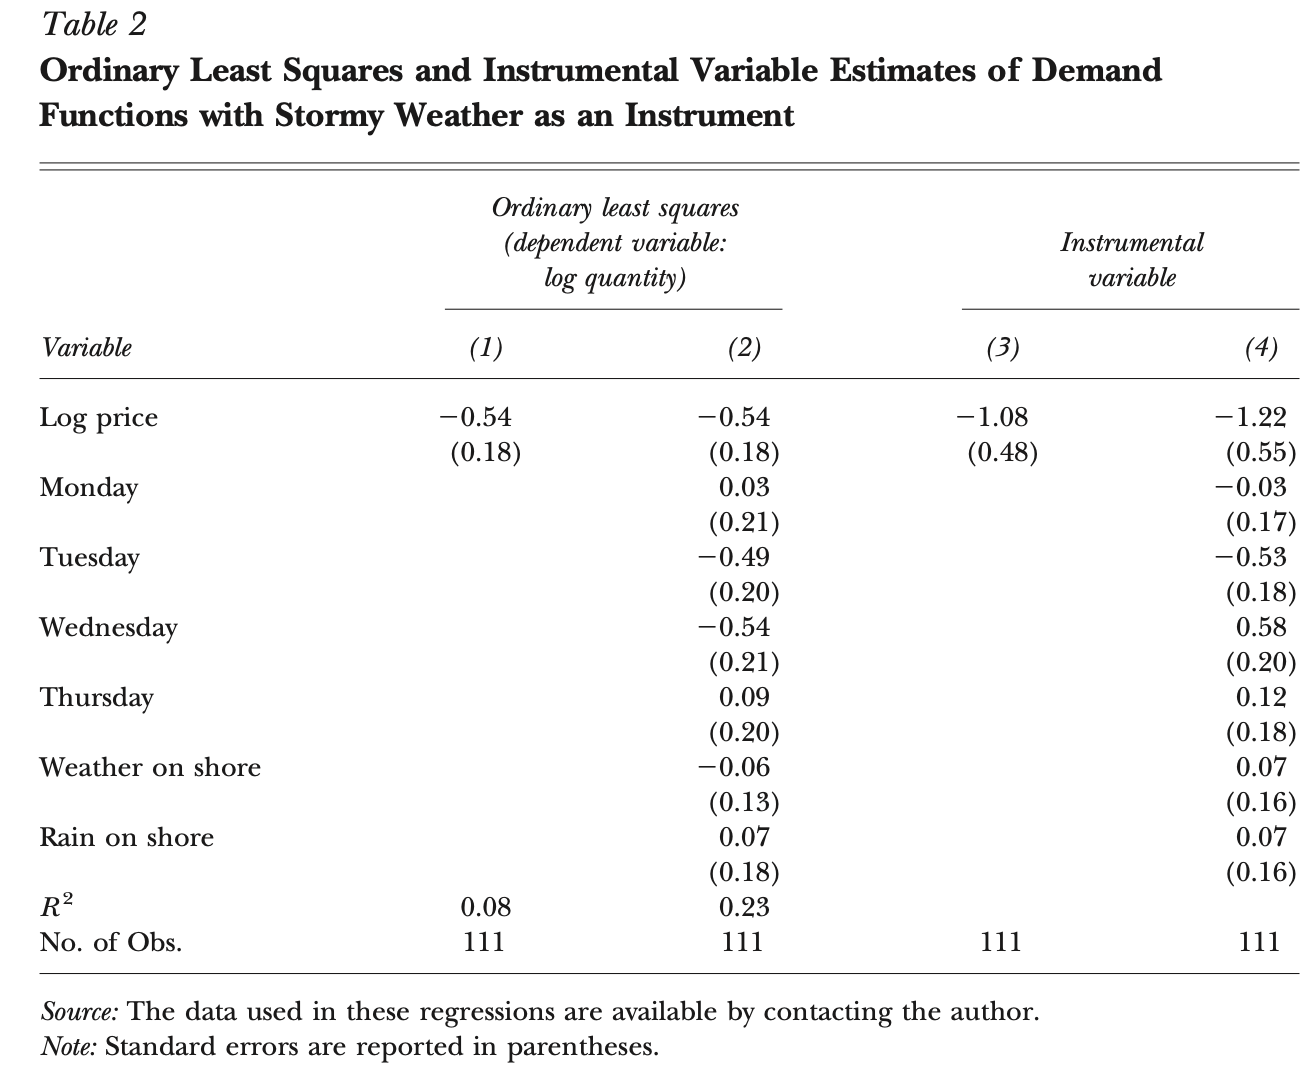
\includegraphics[width=3.5in]{./resources/graddy}
\end{center}

\end{frame}





\begin{frame}{Local Average Treatment Effect}
Finally, we need to understand what monotonicity means in terms of restrictions on economic theory. 
\begin{itemize}
\item To quote from Vytlacil (2002) Econometrica:\\
\emph{ ``The LATE assumptions are not weaker than the assumptions of a latent index model, but instead impose the same restrictions on the counterfactual data as the classical selection model if one does not impose parametric functional form or distributional assumptions on the latter.''}
\item This is important because it shows that the LATE assumptions are equivalent to whatever economic modeling assumptions are required to justify the standard Heckman selection model and has no claim to greater generality.
\item On the other hand there are no magical solutions to identifying effects when endogeneity/selection is present; this problem is exacerbated when the effects are heterogeneous and individuals select into treatment on the basis of the returns.
\end{itemize}
\end{frame}



\end{document}

